\section{Logistic Regression}
In the linear regression we have a linear relationship between the target and the predictors, what if the relationship isn't linear? Let's assume our target is variable is a \textbf{binary variable}
$$
 Y_i=\begin{cases}
 1 & student\ i\ \ passes \\
 0 & student\ i\ \ fails
\end{cases}\ 
\Rightarrow
\prob (Y=1|X=x) = p
$$

If we try to use a linear regression model, we end up with something that ignores the real variable range. 
\begin{figure}[h]
    \centering
    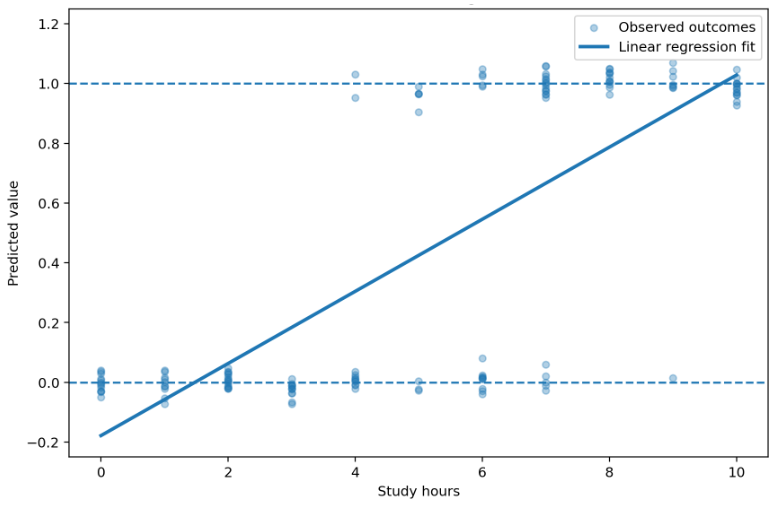
\includegraphics[width=0.3\linewidth]{img/logisticreg/linreg_exced_range.png}
\end{figure}

The idea is to solve the range issue is to change the undeling shape: we shift from the world of probabilities to the world of \textbf{odds} := how more likely is some event to happen with respect to not happen.
$$
 odds = \frac{p}{1-p}
$$
\begin{figure}[h]
    \centering
    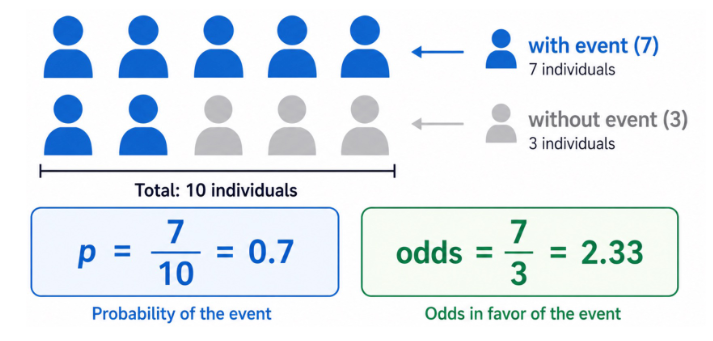
\includegraphics[width=0.3\linewidth]{img/logisticreg/odds_explained.png}
\end{figure}

and we then intepret them as follows:
\begin{itemize}
    \item $odds=1$ success and failure are equally possible
    \item $odds>1$ succcess is more probable than failure 
    \item $odds<1$ failure is more probabl than success
\end{itemize}

However we can't use the linear regression with odds since they are a non-negative measure (the won't never go below zero) \arrow we take instead the \textbf{log-odds/logit}
$$
 \log(odds) = \log\left(\frac{p}{1-p}\right)
$$
\begin{figure}[h]
    \centering
    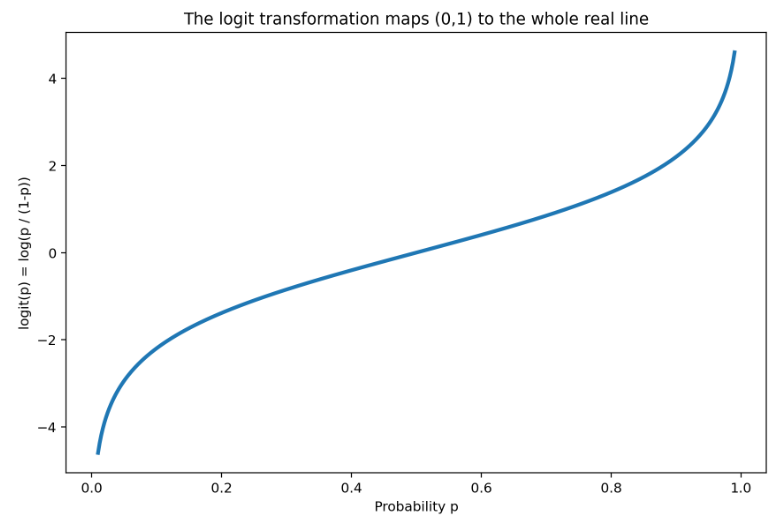
\includegraphics[width=0.3\linewidth]{img/logisticreg/logit_visualized.png}
\end{figure}

Now in this new \textit{log-odds} space we use linear regression:
\begin{align*}    
    & \log(odds) = \log\left(\frac{p}{1-p}\right) = \beta_0 + \beta_1x_{i1}\ ... + \beta_px_{ip}  \\
    & \rightarrow \frac{p_i}{1-p_i} = e^{\beta_0 + \beta_1x_{i1}\ ... + \beta_px_{ip}} \\
    & \rightarrow p_i = \cfrac{1}{1+e^{\beta_0 + \beta_1x_{i1}\ ... + \beta_px_{ip}}}
\end{align*}
so by doing to we get back the probability through the \textbf{linear regression applied within a sigmoid function} (the model is still linear, but in the log-odds scale):
$$
p_i = \sigma(\eta_i)=\sigma(\beta_0+\beta_1x_{i1}...+\beta_px_{ip})
$$
\begin{figure}[h]
    \centering
    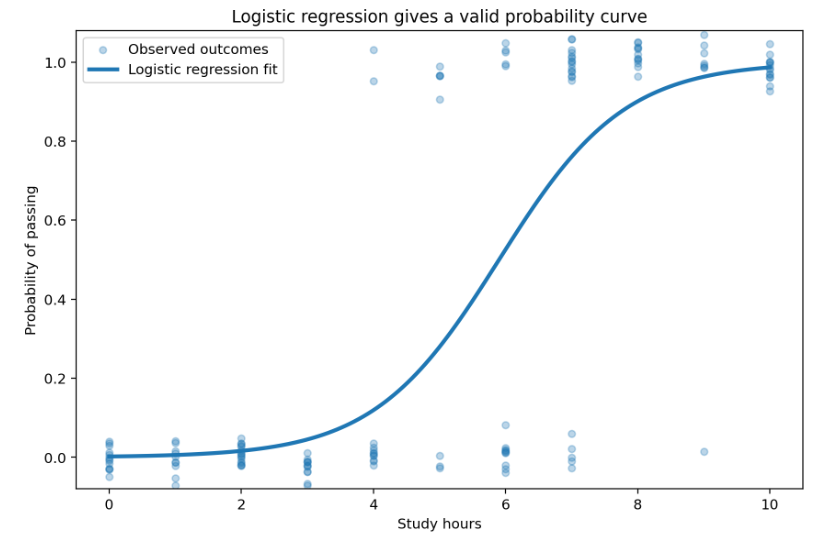
\includegraphics[width=0.5\linewidth]{img/logisticreg/logistic_regression.png}
\end{figure}\hfill\\
One of the advantages of this type fo regression is that it nevere crosses the 0, allowing us to intepret its value as a probability, and instead the extrems flatterns on [0,1]. Another good thing is that we are able to interpret the model:\\

\vspace{0.6cm}
\textbf{Coefficient's interpretation: categorical variables} \\
Our feature is somethign like this:
$$
 x_i=\begin{cases} 0 & GroupA\\ 1& GroupB\end{cases}\ 
\rightarrow \log\left(\frac{p_i}{1-p_i}\right) = \beta_0+\beta_1x_i
$$
to compare the two groups we have to subtract the fitted values:
\begin{align*}
& log\left(\frac{p_B}{1-p_B}\right)-log\left(\frac{p_A}{1-p_A}\right) = \beta_0+\beta_1-\beta_0 = \beta_1 \\
& \\
& \rightarrow \log\left(\frac{p_b/(1-p_B)}{p_A/(1-p_A)}\right)=\beta_1
\end{align*}
$\Rightarrow$ the odds-ratio is equal to the slope in the log-odds space.

\newpage
\textbf{Coefficient's intereptation: continuous variables}\\
If instead we consider a continuous predictor we get
\begin{align*}
& \log\left(\frac{p(x)}{1-p(x)}\right)=\beta_0+\beta_1x,\ \log\left(\frac{p(x+1)}{1-p(x+1)}\right)=\beta_0+\beta_1(x+1) \\
& \\
& \rightarrow \log\left(\frac{odds\ at\ x+1}{odds\ at\ x}\right) = \beta_1
\end{align*}

Also in the continouous case $e^{\beta_1}$ is the odds-ratio for single-unit increase. 
In general we can deduce that the increase is constant in the log-odds space:
\begin{figure}[h!]
    \centering
    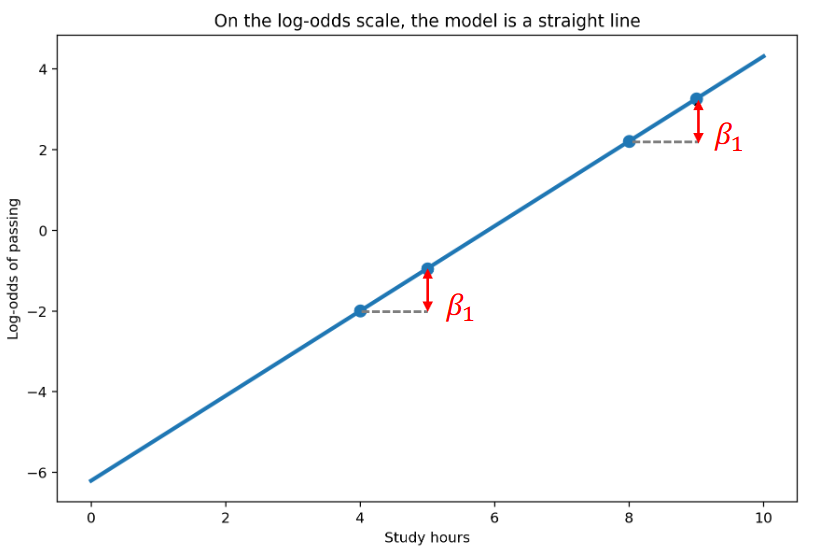
\includegraphics[width=0.4\linewidth]{img/logisticreg/logodds_slope.png}
\end{figure}

The the effect in the odds space is still constant $e^{\beta_1}$, but visualized as an exponential:
\begin{figure}[h]
    \centering
    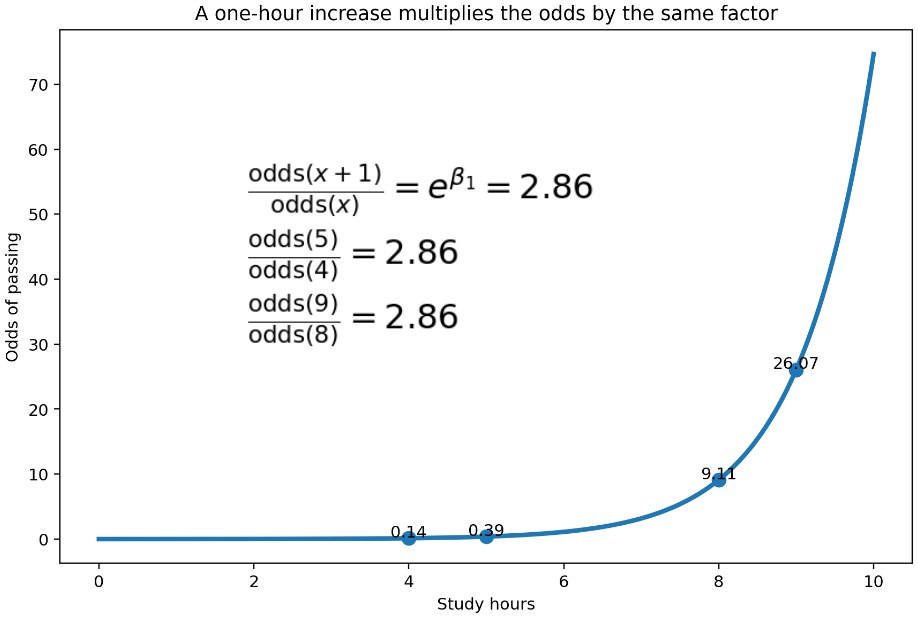
\includegraphics[width=0.4\linewidth]{img/logisticreg/odds_slope.png}
\end{figure}

On probablities instead the ratio is not constant, but dependes on where the position on the logistic curve:
\begin{figure}[h]
    \centering
    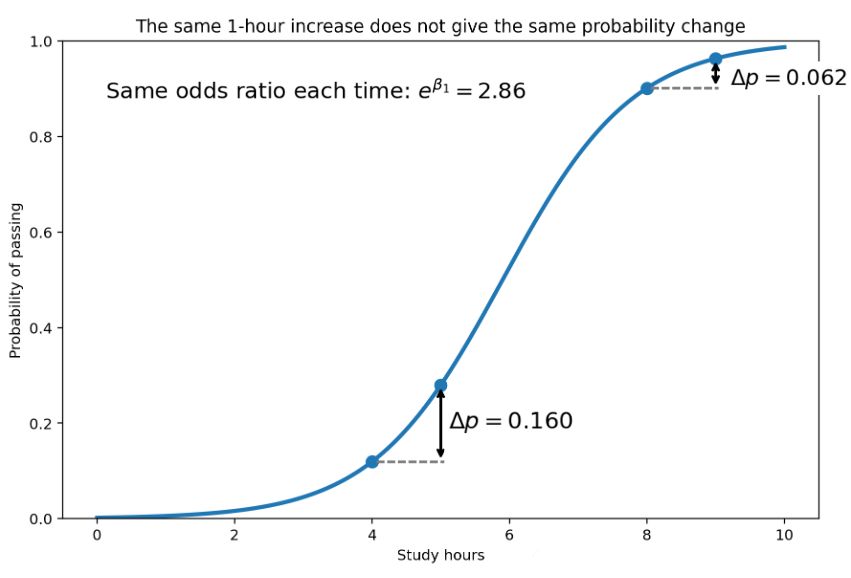
\includegraphics[width=0.5\linewidth]{img/logisticreg/prob_logreg_slode.png}
\end{figure}

\newpage
% --------------------------------------------------------------------------------------------------------
\subsubsection{Generalized Linear Models (GLM)}
Linear regression is a specific case of GLM, which is a generalization of linear regression that links the linear model with the response through a non-linear \textbf{linking function} $g$.

We can always identify three elements:
\begin{enumerate}
    \item random response variables
    \item linear model of the predictors $\eta_i=\beta_0+\beta_1x_{i1}...+\beta_px_ip{}$
    \item linking function $g(\mu_i)=\eta_i$ where $\mu_i=\mathbb{E}[Y_i|X_i]$
\end{enumerate}
To get the basic linear regression model from GLMS, we can take $g()=Id$


% --------------------------------------------------------------------------------------------------------
\vspace{0.3cm}
\subsection{Classification models (classifiers)}
The logistic regression doesn't give a label directly, instead its output is the probability of that label: $\hat{p}_i=\mathbb{P}(Y_i=1|X_i)$.
To get some kind of \textbf{classification rule} we have to set a \textit{treshold} $t\in (0,1)$
$$
\hat{Y}_i=\begin{cases}
    1 & \hat{p_1}\ge t \\
    0 & \hat{p_1}< t 
\end{cases}
$$
\begin{figure}[h]
    \centering
    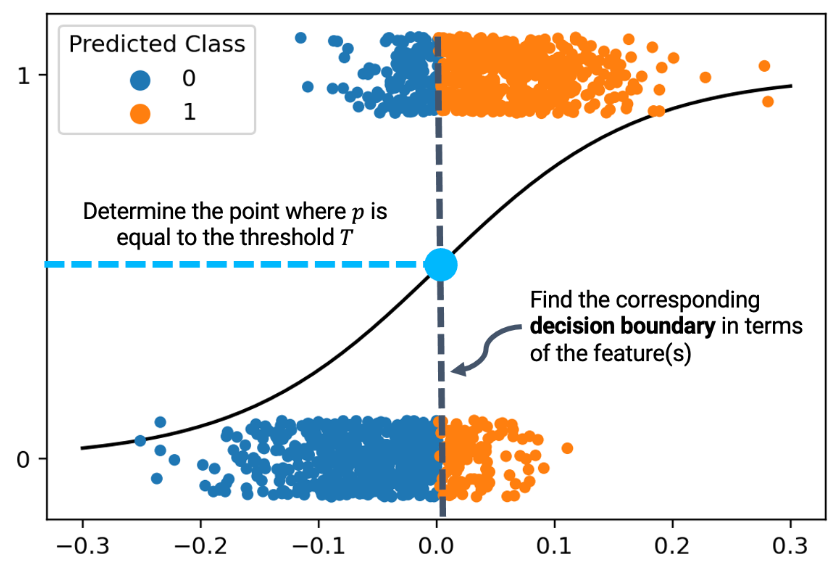
\includegraphics[width=0.4\linewidth]{img/logisticreg/logreg_classificator.png}
\end{figure}

\paragraph{How to choose the threshold}
The most common choice is taking $t=0.5$, however is really context-dependent: if we'd like a model more selective/conservative we should take a high treshold.
Sometimes when the datset is \textit{unbalanced} it might be a good idea to set the treshold to the relative frequence of the minority class. Another suggestion is to use the \textit{negative class} frequency (by convention the case $0$ is the negative class) . Otherwise there is also the \textit{Youden's J index} which suggest of using $TPR -FPR$ (see later what this values are).

% --------------------------------------------------------------------------------------------------------
\vspace{0.3cm}
\subsection{Model assumption of linear regression}
Some assumption made for the linear regression moels are relaxed, for the logistic regression usually we assume that:
\begin{itemize}
    \item observations are independet
    \item only important/meaningful predictors are included, irrelvant ones arent't added
    \item there is no multicollinearity
    \item the logit event probability is linear in the predictors
    \item there is no \textbf{perfect separation} := there is no variable that divides perfecly the dataset in classes
\end{itemize}

\newpage
However we can handle easily also \textbf{interactions among predictors} (bilinear relationships).\\
If we take as exmaple $x_{i1}$ = study hours, $x_{i2}$ = good/bad sleep we get as model
$$
\log\left(\frac{p_i}{1-p_i}\right)=\beta_0+\beta_1 x_{i1} +\beta_2 x_{i2} +\beta_3 x_{i1} x_{i2}
$$
by fixing the value of one varibale we can study the behavior of the model when the other predictor changes, obtaining two different reduced models with \textit{diffrent slopes}
\begin{figure}[h]
    \centering
    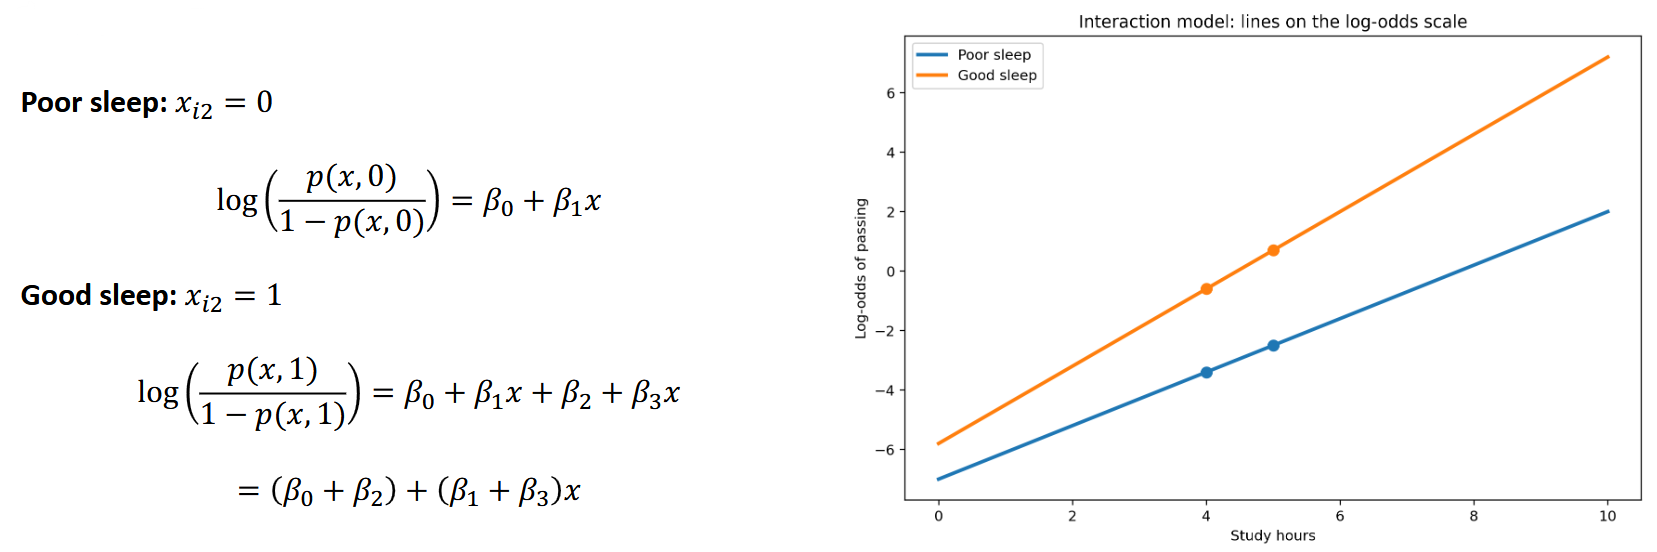
\includegraphics[width=0.8\linewidth]{img/logisticreg/partial_model.png}
\end{figure}\hfill\\
this different slope in the log-odds space is reflected also in the probability space, getting two different probability curves:
\begin{figure}[h]
    \centering
    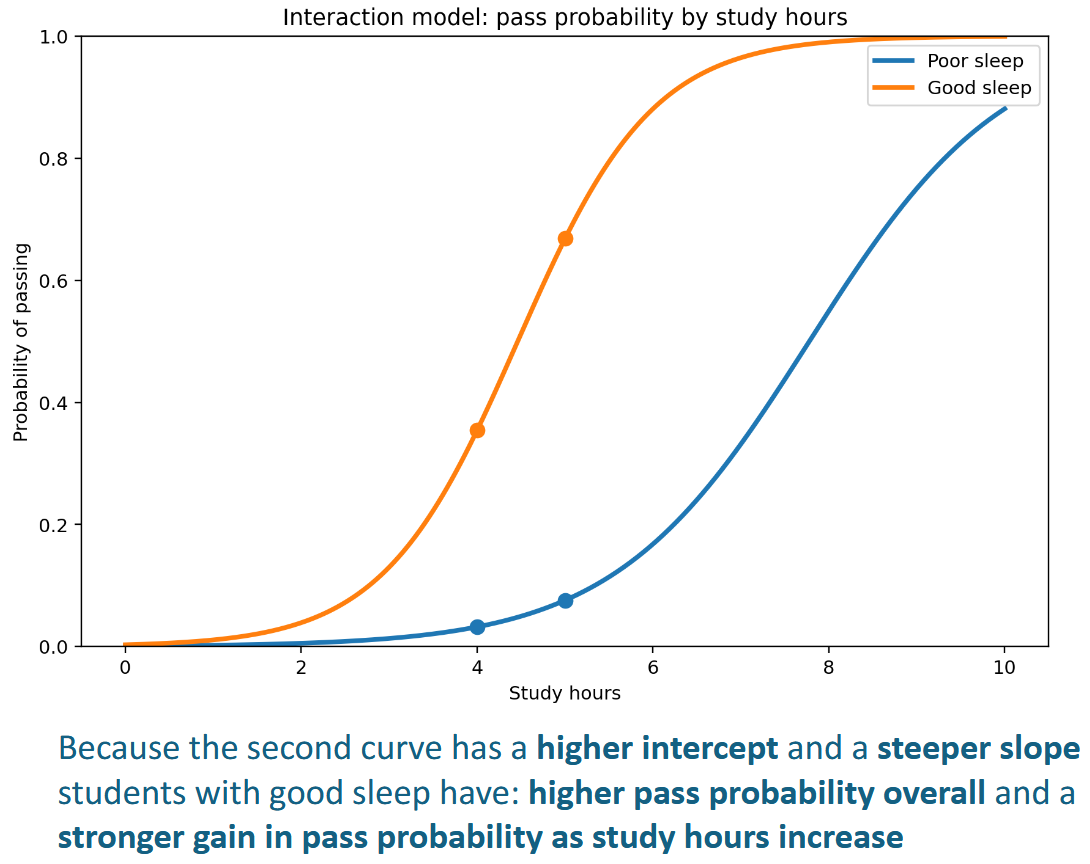
\includegraphics[width=0.5\linewidth]{img/logisticreg/logreg_probs_interacting_vars.png}
\end{figure}

% --------------------------------------------------------------------------------------------------------
\vspace{0.3cm}
\subsection{Logistic model estimation}
Since our predictors are binary $\{0,1\}\ni Y_i \sim Bernoulli(p_i)$ we have that $\prob(Y_i=y|X_i)=p_i^{y}(1-p_i)^{1-y}$ \arrow a good model should assing high probability to the outcomes that actually occurred and low to those not occurred \arrow a good model chooses $\beta$s so that the observed pattern are as plausible as possible.\\ 
To estimate the model we use MLE as always:
$$
L(\beta)= \prod_{i=1}^np_i^y(1-p_i)^{1-y} \rightarrow \ell(\beta)=\log L(\beta) = \sum_{i=1}^n y\log p_i + (1-y)\log (1-p_i
$$

\newpage
\subsubsection{Estimation with perfect separation}
Perfect separation occours when some predictor divides the two classes completely. While might looks like a good thing, it's a little bit tricky for the MLE: likelihood makes the logistic curve steeper and steeper, approaching the step function, and this would require the estimation of an infinite estimator, which is not possible with MLE.
\begin{figure}[h]
    \centering
    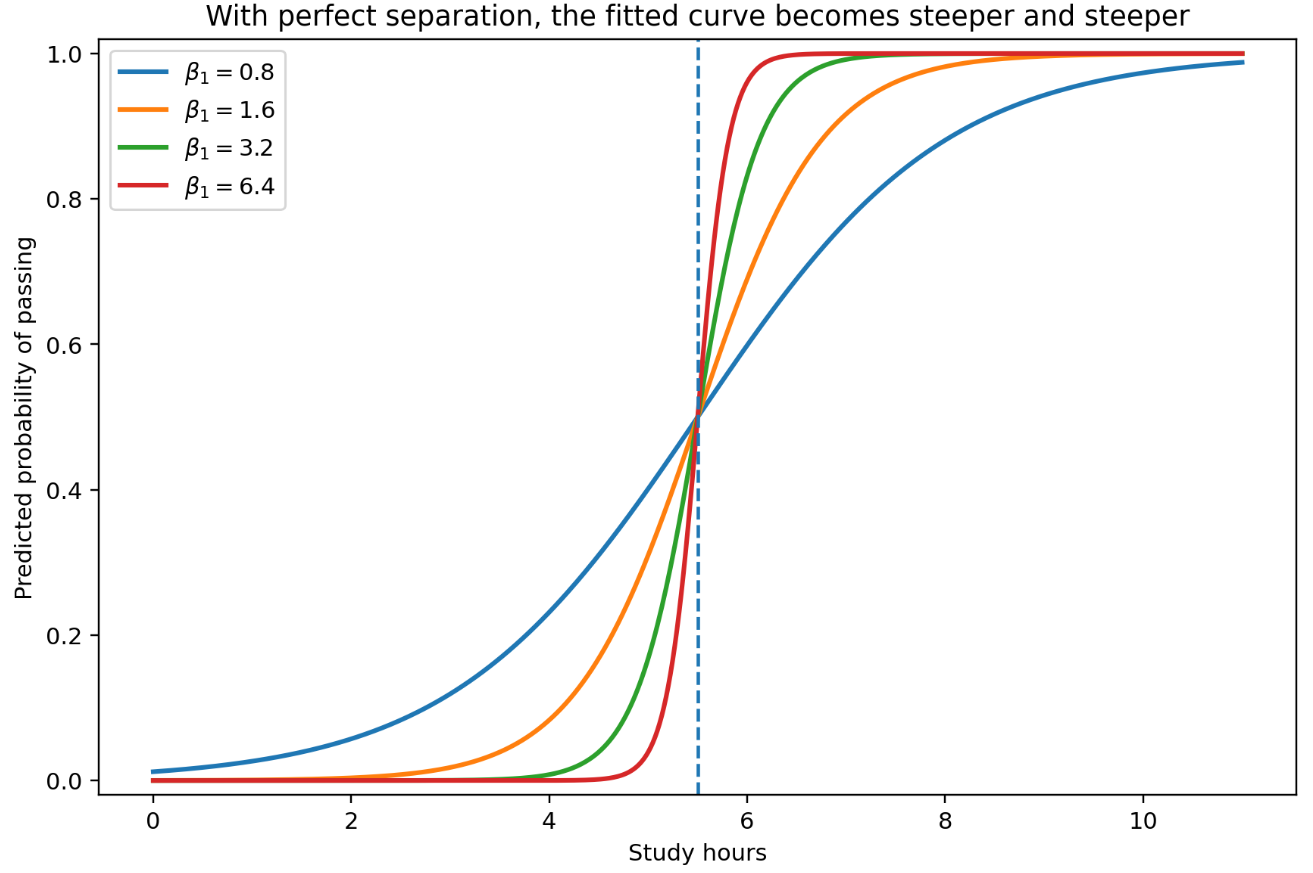
\includegraphics[width=0.4\linewidth]{img//logisticreg/mle_perfect_sep.png}
\end{figure}
\hfill\\
Similar situation for the \textbf{quasi-complete separation} := most predictors are perfectly separated but a small group overlap. In this setting the fitted coefficients might suffer from unstability.\\
\hfill\\
In the case of (quasi)perfect separation software might fail to converge, return extremely large coefficients with large std errors, or in some cases even warnings. To avoid these isseus we can try to collect more data, simplifying the model, combine/remove sparse categories or use penalized logistic regression (logistic regression that adds penalties in the loss function to avoid overfitting).

% --------------------------------------------------------------------------------------------------------
% give another look to this
\vspace{0.3cm}
\subsection{Model usefulness assessment}
A first approach to measure our model's performance is compare it with the purely-random/intercept-only predictor. As metric for the comparison we use the \textbf{likelihood ratio test} 
$$
2(\ell_{full}-\ell_{null})
$$ 
where $full$ stand for our model and $null$ for the intercept-only \arrow the larger the better. The 2 is only to fit the statistic in a Chi-squared distribution.\\

\vspace{0.5cm}
Another metric to evaluate our model il the \textbf{deviance} $-2\ell$ where $\ell$ is the log-likelihood, so the larger the better.\\
This statistic is useful when we want to compare two nested models.

\vspace{0.5cm}
Another metric used to compare out model with the intercept-only one we can also use the \textbf{McFdadden's pseudo-$R^2$}
$$
R^2_{McFadden}  = 1 -\cfrac{\ell_{full}}{\ell_{null}}
$$

After general model fitting estimation, we'd like to know whether each predicotr contributes or not: to do so we use statistic tests: $H_0:\beta_j=0$ vs $H_1:\beta_j\neq0$\\
A common used statistic is
$$
z=\cfrac{\hat{\beta}_j}{SE(\hat{\beta}_j)}
$$
if the values is large then the realtive p-value is low, giving strong evidence that the predictor is meaningful. As usual, if we build a confidence interval we get $\hat{\beta}_j \pm z_{1-\alpha/2}\ SE(\hat{\beta}_j)$ and this interval contains zero, the coefficient might be absent.
However this is for the log-odds, for the odds realm we have to make it exponential:
$$
\hat{\beta}_j \rightarrow e^{\hat{\beta}_j},\ \left[e^{\hat{\beta}_j^L}\ ,\ e^{\hat{\beta}_j^U} \right]
$$
if this interval in the odds world contains 1 hten the coefficient might be irrelevant.

% --------------------------------------------------------------------------------------------------------
\subsection{Classifier performance}
We can resume the outcome ouf our classfier in a \textbf{confusion matrix}: it resumes the outcome of the model in predicting the datapoint classification.
\begin{figure}[h]
    \centering
    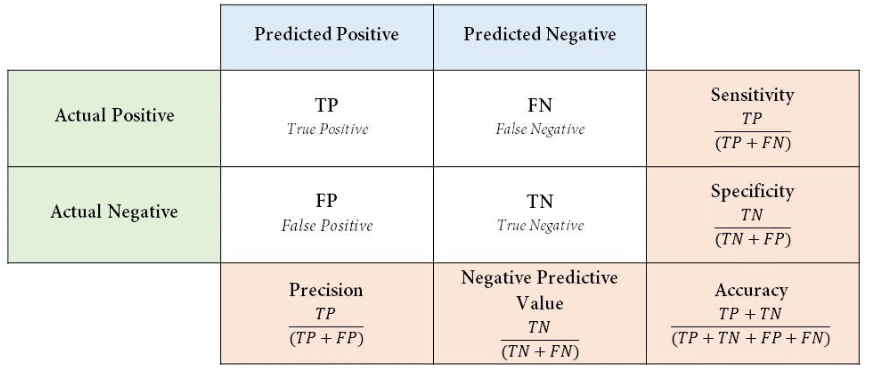
\includegraphics[width=0.6\linewidth]{img/logisticreg/classifier_performance.png}
\end{figure}\hfill\\
\textbf{Accuracy} := raw number of good evaluation, a little bit silly since is influenced by how much tha dataset is unbalanced.

% take the last 5-10 minutes of the recording in which she's talking about the ROC curve and AUC index, plus

We could see that these values are dependent from the threshold chosen. We could think of maximizing the model selection based on the maximization of accuracy.

To remove this dependecy we can take the area of this curve.

This type of evaulation for classification model has some drawbacks: it requires amodel that uses probabilities as output.
% -----
Other metrics are 
$$\text{Recall} = \text{Sensitivity} = \frac{TP}{TP+FN}$$
$$\text{F1-Score} = \frac{2 \cdot \text{Precision} \cdot \text{Recall}}{\text{Precision} + \text{Recall}}$$
$$\text{Specificity} = \frac{TN}{TN+FP}$$